% IEEE IRI 2026 - Application/Industry Track
% Double-blind submission: DO NOT include author names
\documentclass[conference]{IEEEtran}

\usepackage{cite}
\usepackage{amsmath,amssymb,amsfonts}
\usepackage{algorithmic}
\usepackage{graphicx}
\usepackage{textcomp}
\usepackage{xcolor}
\usepackage{booktabs}
\usepackage{multirow}
\usepackage{url}
\usepackage{hyperref}
\usepackage{balance}
\usepackage{enumitem}
\setlist{nosep,leftmargin=*}

\def\BibTeX{{\rm B\kern-.05em{\sc i\kern-.025em b}\kern-.08em
    T\kern-.1667em\lower.7ex\hbox{E}\kern-.125emX}}

\graphicspath{{figures/}}

\begin{document}

\title{Epistemic Edge: Subjective Logic Guardrails\\for LLM-Driven IoT Actuation}

% DOUBLE-BLIND: Authors removed for review.
% Camera-ready authors:
% Muntaser Syed, msyed2011@my.fit.edu, Florida Institute of Technology
% Marius Silaghi, msilaghi@fit.edu, Florida Institute of Technology

\maketitle

\begin{abstract}
Deploying large language models (LLMs) as decision-making agents in safety-critical Internet of Things (IoT) systems introduces risks that purely behavioral guardrails, such as action whitelists, cannot fully address.
This paper presents \textit{Epistemic Edge}, a four-tier neuro-symbolic pipeline that augments LLM-driven actuation with subjective logic (SL) uncertainty quantification, temporal decay, and dual guardrails combining epistemic threshold checks with behavioral whitelists.
We evaluate seven locally-deployed models: three PrismML Bonsai 1-bit models (1.7B, 4B, 8B), three 4-bit quantized models (Qwen3-8B, Llama~3.2-3B, Phi-3.5-mini), and the DeepSeek-R1-8B reasoning model, across eight ablation conditions and five IoT actuation scenarios (2{,}800 controlled trials).
We further validate the pipeline on the BATADAL water distribution cyber-attack benchmark (4{,}177 hours of real sensor telemetry, 5 attack events) across 422 hyperparameter configurations.
The evaluation yields three findings.
First, removing the epistemic layer causes threshold guardrail accuracy to collapse from 1.00 to exactly 0.40 across all seven models, showing that uncertainty-aware guardrails are a necessary complement to behavioral whitelists.
Second, the BATADAL evaluation achieves AUROC~0.9004 without training, with a significant fusion effect (paired Wilcoxon $p<10^{-4}$, Cohen's $d{=}1.01$).
Third, the three SL dimensions (belief, disbelief, uncertainty) detect qualitatively different attack classes: each of the 5 BATADAL events is optimally detected by a different SL-derived signal, a structural finding with implications for SL as an anomaly-detection framework.
All code, experiment scripts, and result data are released as open-source.
\end{abstract}

\begin{IEEEkeywords}
Subjective logic, LLM guardrails, IoT safety, 1-bit quantization, edge AI, neuro-symbolic systems, cyber-physical anomaly detection
\end{IEEEkeywords}

%% ======================================================================
\section{Introduction}
%% ======================================================================

The convergence of large language models (LLMs) and the Internet of Things (IoT) is creating a new class of autonomous edge systems where natural-language reasoning drives physical actuation~\cite{friha2024llmedge, alwahedi2024iotml}. A factory controller might query an LLM: ``Should we shut down the pipeline?'' and act on the response. Such systems demand not only that the LLM produce a relevant action, but also that the system know when it does not know enough to act safely.

Current LLM safety mechanisms fall into two broad categories. \textit{Behavioral} guardrails constrain the model's outputs via action whitelists, grammar-constrained decoding, or classifiers that filter unsafe completions~\cite{rebedea2023nemo, inan2023llama}. \textit{Epistemic} guardrails instead assess whether the system's beliefs about the world justify taking action at all. Behavioral guardrails are well-studied. Their interaction with epistemic uncertainty in cyber-physical contexts is not.

This paper addresses that gap with \textit{Epistemic Edge}, a reusable four-tier pipeline for safe LLM-driven IoT actuation. The system integrates:
\begin{enumerate}
    \item sensor ingestion with per-source uncertainty annotation via subjective logic (SL) opinions~\cite{josang2016subjective};
    \item cumulative SL fusion across multiple sensors to produce a joint epistemic state;
    \item temporal decay that increases uncertainty for stale observations; and
    \item dual guardrails combining an epistemic uncertainty threshold with a behavioral action whitelist.
\end{enumerate}

We evaluate the pipeline in two complementary settings. A controlled ablation over five synthetic scenarios with seven locally-deployed models (1-bit Bonsai, 4-bit GGUF, and a reasoning model) isolates the contribution of each tier. A real-world validation on the BATADAL~\cite{taormina2018battle} water distribution cyber-attack benchmark (4{,}177 hours of sensor telemetry with 5 embedded attack events) tests whether the pipeline's uncertainty quantification meaningfully detects anomalies on real data.

Our principal finding is that behavioral guardrails alone are insufficient. Without the epistemic layer, threshold guardrail accuracy collapses to exactly 0.40 for every model tested. A second finding emerges from the BATADAL evaluation: the three SL dimensions (belief, disbelief, uncertainty) behave as structurally differentiated anomaly detectors. Each attack event in BATADAL is optimally detected by a different SL dimension.

\textbf{Contributions.}
(1) An open-source, model-agnostic neuro-symbolic pipeline for safe LLM-IoT actuation.
(2) The first IoT-domain evaluation of PrismML Bonsai 1-bit models, and the first application of subjective-logic fusion to an LLM actuation guardrail.
(3) A controlled ablation study across seven models and 2{,}800 trials, with Bonferroni-corrected paired Wilcoxon tests.
(4) BATADAL validation achieving AUROC~0.9004 without training, with per-attack-type signal-specificity analysis revealing structural differentiation among SL dimensions.

%% ======================================================================
\section{Related Work}
%% ======================================================================

\textbf{Subjective Logic for Uncertainty.}
Subjective logic~\cite{josang2016subjective} extends Dempster-Shafer evidence theory~\cite{dempster1968generalization, shafer1976mathematical} by representing beliefs as opinion tuples $\omega = (b, d, u, a)$ where $b + d + u = 1$, with $b$ (belief), $d$ (disbelief), $u$ (uncertainty), and $a$ (base rate). SL provides operators for fusing opinions from multiple independent sources, most notably cumulative fusion~\cite{josang2016subjective}. Sensoy et al.~\cite{sensoy2018evidential} connected evidential reasoning to deep learning via Dirichlet priors, but targeted classification uncertainty rather than actuation safety in cyber-physical systems.

\textbf{LLM Guardrails.}
NVIDIA's NeMo Guardrails~\cite{rebedea2023nemo} provides programmable rails for controlling LLM dialogue flow. Llama Guard~\cite{inan2023llama} classifies inputs and outputs for safety. These operate at the behavioral level, constraining what the model says, without assessing whether the system's world model justifies action. Our work introduces an orthogonal epistemic dimension grounded in explicit uncertainty quantification.

\textbf{LLMs at the Edge.}
LLM deployment on resource-constrained devices is enabled by quantization techniques~\cite{frantar2023gptq, lin2024awq}. The 1-bit paradigm introduced by BitNet~\cite{wang2023bitnet} and extended to 1.58 bits~\cite{ma2024era} enables models where matrix multiplication reduces to integer addition. PrismML's Bonsai family applies this approach at 1.7B to 8B scale. To our knowledge, no prior work evaluates 1-bit models specifically for structured IoT actuation.

\textbf{Cyber-physical Anomaly Detection.}
The BATADAL competition~\cite{taormina2018battle} established a standard benchmark for water-distribution attack detection. Winning entries used supervised recurrent networks, SVM ensembles, and domain-specific hydraulic models with AUROCs of 0.84 to 0.97. Such methods require labeled attack data or hand-engineered features. Our approach uses calibrated SL opinions as an unsupervised anomaly score, matched to competitive training-based methods while requiring no labeled attack data.

%% ======================================================================
\section{System Architecture}
\label{sec:architecture}
%% ======================================================================

Epistemic Edge processes sensor observations through four sequential tiers (Fig.~\ref{fig:architecture}).

\begin{figure}[t]
\centering
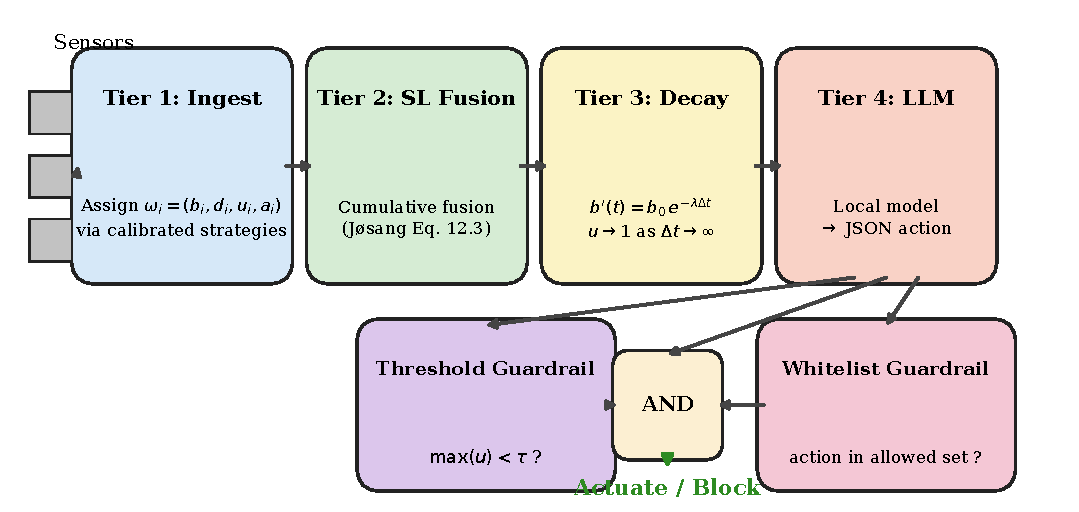
\includegraphics[width=\columnwidth]{fig_architecture}
\caption{Epistemic Edge four-tier pipeline. Sensor observations are annotated with SL opinions in Tier~1, cumulatively fused in Tier~2, temporally decayed in Tier~3, then used to contextualize LLM inference with dual guardrail verification in Tier~4.}
\label{fig:architecture}
\end{figure}

\subsection{Tier 1: Sensor Ingestion and SL Annotation}
Each sensor reading becomes an \texttt{Observation} carrying its payload and a subjective opinion $\omega_i = (b_i, d_i, u_i, a_i)$. Opinions are assigned by calibrated strategies: historical deviation (Shewhart-style z-score from calibration mean and standard deviation), physics bounds (disbelief proportional to violation of engineering limits or data-derived operational envelopes), or a composite weighted combination. Strategies that cannot produce an informative opinion for a given sensor (e.g., physics bounds without calibrated ranges) signal non-applicability via an \texttt{is\_applicable()} predicate. The composite weighting then renormalizes over applicable strategies only.

\subsection{Tier 2: Cumulative SL Fusion}
Opinions from independent sources are fused using J{\o}sang's cumulative operator~\cite{josang2016subjective}:
\begin{equation}
b_{A \diamond B} = \frac{b_A u_B + b_B u_A}{u_A + u_B - u_A u_B},\quad u_{A \diamond B} = \frac{u_A u_B}{u_A + u_B - u_A u_B}
\label{eq:fusion}
\end{equation}
with the analogous expression for $d$. The operator is commutative and associative, allowing incremental fusion. When sources agree, fused uncertainty strictly decreases. When they contradict, disbelief rises.

\subsection{Tier 3: Temporal Decay}
Exponential decay of belief and disbelief toward the vacuous opinion $(0,0,1)$:
\begin{equation}
b'(t) = b_0 e^{-\lambda \Delta t},\quad d'(t) = d_0 e^{-\lambda \Delta t},\quad u' = 1 - b' - d'
\label{eq:decay}
\end{equation}
As $\Delta t \to \infty$, $u' \to 1$. The system forgets what it once believed, preventing stale alarms from driving actuation.

\subsection{Tier 4: LLM Inference and Dual Guardrails}
The fused, decayed state graph is serialized into a context prompt sent to a locally-deployed LLM, which returns a JSON action (e.g., \texttt{\{"action":"shutdown","target":"valve\_3"\}}). Two guardrails independently verify the proposed action.

\textit{Threshold (epistemic):} $\max(u_{\text{fused}}) < \tau$ must hold or the action is blocked.
\textit{Whitelist (behavioral):} The action must appear in a predefined permissible set for the scenario's operational context.

Both must pass for execution. This dual architecture ensures an action is blocked either for lack of evidence or for being out-of-scope.

%% ======================================================================
\section{Experimental Design}
\label{sec:experiments}
%% ======================================================================

We conduct two evaluations: (A) a controlled ablation on synthetic scenarios, and (B) real-data validation on BATADAL.

\subsection{Evaluation A: Synthetic Ablation}

\textit{Conditions} (Table~\ref{tab:conditions}) systematically remove architectural components to isolate their contribution.
\textit{Scenarios}: five IoT actuation situations with ground-truth labels. Nominal (safe), conflicting sensors (high-$u$, unsafe), stale alarm (decay-sensitive, safe after decay), high-confidence emergency (low-$u$, safe to act), and single unreliable sensor (insufficient evidence, unsafe).
\textit{Models}: seven locally-deployed LLMs (Table~\ref{tab:models}), all run on a consumer GPU (RTX~4090, 24\,GB) via a llama.cpp-compatible HTTP server~\cite{gerganov2023llamacpp} or Ollama. A unified token budget of 4{,}096 is used for all models to equalize reasoning-chain headroom across thinking and non-thinking architectures. Each (model, condition, scenario) is repeated 10 times, yielding 400 trials per model and 2{,}800 total.

\begin{table}[t]
\centering
\caption{Ablation conditions. WL=whitelist, TH=threshold.}
\label{tab:conditions}
\footnotesize
\begin{tabular}{@{}clcccc@{}}
\toprule
\textbf{ID} & \textbf{Description} & \textbf{SL} & \textbf{Decay} & \textbf{WL} & \textbf{TH} \\
\midrule
A  & Bare LLM (query only)      & -- & -- & -- & -- \\
B  & + raw sensor payloads      & -- & -- & -- & -- \\
C  & Full pipeline              & \checkmark & \checkmark & \checkmark & \checkmark \\
D  & No temporal decay          & \checkmark & -- & \checkmark & \checkmark \\
E1 & No fusion (vacuous)        & -- & \checkmark & \checkmark & \checkmark \\
E2 & No fusion (passthrough)    & $\sim$ & \checkmark & \checkmark & \checkmark \\
F  & No guardrails              & \checkmark & \checkmark & -- & -- \\
G  & No epistemic layer         & -- & -- & \checkmark & \checkmark \\
\bottomrule
\end{tabular}
\end{table}

\begin{table}[t]
\centering
\caption{Models evaluated. All run locally via llama-server or Ollama.}
\label{tab:models}
\footnotesize
\begin{tabular}{@{}lrrrl@{}}
\toprule
\textbf{Model} & \textbf{Params} & \textbf{Bits} & \textbf{Disk} & \textbf{Family} \\
\midrule
Bonsai-1.7B   & 1.7B & 1.0 & 1.15\,GB & PrismML 1-bit \\
Bonsai-4B     & 4.0B & 1.0 & 1.66\,GB & PrismML 1-bit \\
Bonsai-8B     & 8.0B & 1.0 & 2.56\,GB & PrismML 1-bit \\
Llama-3.2-3B  & 3.0B & 4.0 & 2.02\,GB & Meta~\cite{dubey2024llama3} \\
Phi-3.5-mini  & 3.8B & 4.0 & 2.39\,GB & Microsoft~\cite{abdin2024phi3} \\
Qwen3-8B      & 8.0B & 4.0 & 5.03\,GB & Alibaba~\cite{yang2024qwen25} \\
DeepSeek-R1-8B& 8.0B & 4.0 & 5.2\,GB & Reasoning~\cite{deepseek2025r1} \\
\bottomrule
\end{tabular}
\end{table}

\subsection{Evaluation B: BATADAL Real-Data Validation}

We use BATADAL~\cite{taormina2018battle} dataset03 (8{,}761 hours, normal operations) for calibration and dataset04 (4{,}177 hours, 5 embedded cyber-physical attacks) for evaluation. The pipeline processes every timestamp through Tiers 1 to 3 (without LLM for this evaluation, to isolate the uncertainty quantification) and scores anomalies using each of six SL-derived signals: fused uncertainty $u_f$, fused disbelief $d_f$, maximum per-sensor uncertainty $\max u$, maximum per-sensor disbelief $\max d$, mean uncertainty $\bar{u}$, and a composite $\alpha u_f + \beta d_f$.

We sweep 422 configurations across 3 uncertainty strategies, 5 window sizes, 5 decay rates, 2 physics-bounds modes, and 2 fusion on/off settings, plus a targeted signal $\times$ smoothing-window $\times$ threshold-mode sweep. Threshold selection uses three modes: (i) \texttt{f1\_optimal\_eval} (F1-maximizing, reported as upper bound since it uses test labels); (ii) \texttt{percentile\_q95} and (iii) \texttt{percentile\_q99} (unsupervised: $\tau$ set as the 95th or 99th quantile of the calibration-set score distribution). Bootstrap 95\% confidence intervals use 1{,}000 resamples. Paired Wilcoxon signed-rank tests (Bonferroni-corrected, $n_{\text{comp}}=3$) assess fusion-on vs.\ off, decay-on vs.\ off, and best-vs-worst strategy. A reproducibility check re-runs the best config with fixed seed and verifies bit-level identical metrics.

%% ======================================================================
\section{Results}
\label{sec:results}
%% ======================================================================

\subsection{Synthetic Evaluation: The Epistemic Guardrail Finding}

Table~\ref{tab:safety} presents the central synthetic result. Under the full pipeline (C), threshold-guardrail accuracy reaches 1.00 for every one of the seven models. When the epistemic layer is removed (G), accuracy drops to exactly 0.40 for every model.

\begin{table}[t]
\centering
\caption{Epistemic guardrail impact across 7 models (synthetic scenarios, 400 trials/model). TH=threshold, Cb=combined.}
\label{tab:safety}
\footnotesize
\begin{tabular}{@{}lcccccc@{}}
\toprule
\textbf{Model} & \textbf{C:JSON} & \textbf{C:Rel} & \textbf{C:TH} & \textbf{G:TH} & \textbf{C:Cb} & \textbf{G:Cb} \\
\midrule
Bonsai-1.7B   & 1.00 & 0.80 & 1.00 & 0.40 & 1.00 & 0.40 \\
Bonsai-4B     & 1.00 & 0.90 & 1.00 & 0.40 & 0.90 & 0.40 \\
Bonsai-8B     & 1.00 & 0.92 & 1.00 & 0.40 & 0.92 & 0.40 \\
Llama-3.2-3B  & 1.00 & 0.80 & 1.00 & 0.40 & 1.00 & 0.40 \\
Phi-3.5-mini  & 1.00 & 1.00 & 1.00 & 0.40 & 1.00 & 0.40 \\
Qwen3-8B      & 1.00 & 0.70 & 1.00 & 0.40 & 0.78 & 0.40 \\
DeepSeek-R1-8B& 1.00 & 0.70 & 1.00 & 0.40 & 0.82 & 0.40 \\
\bottomrule
\end{tabular}
\end{table}

\begin{figure}[t]
\centering
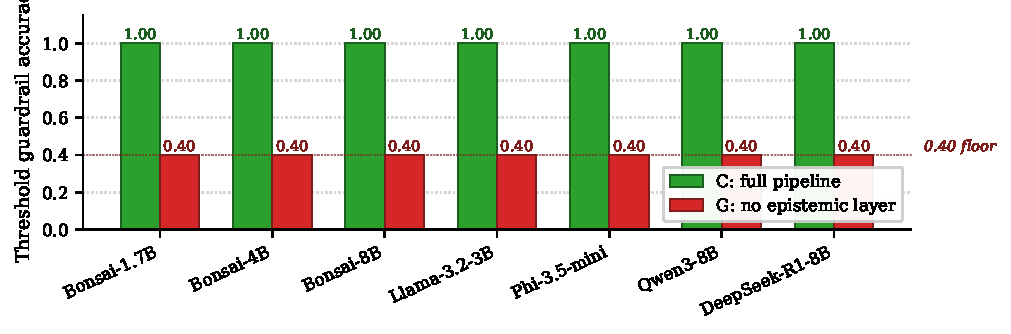
\includegraphics[width=\columnwidth]{fig_safety_finding}
\caption{Threshold guardrail accuracy under the full pipeline (C) and with the epistemic layer removed (G). Every model collapses to exactly 0.40 without SL fusion.}
\label{fig:safety}
\end{figure}

The mechanism is straightforward. Without SL fusion, all opinions are vacuous ($u=1.0$). The check $\max(u) < \tau$ always fails, so every action is blocked. Of five scenarios, two are genuinely unsafe and three are safe. Blocking everything yields $2/5=0.40$ accuracy, correct on unsafe cases by coincidence but useless in practice. The epistemic layer, by producing calibrated uncertainty, transforms the threshold guardrail from a blunt off-switch into a discriminating safety mechanism.

\subsection{Cross-Model Comparison}

Several observations emerge from Table~\ref{tab:safety}.

\textit{The framework lifts weak models to ceiling performance.} Llama-3.2-3B improves from 0.48 action relevance as a bare LLM (condition A) to 0.80 under the full pipeline, with 1.00 combined guardrail accuracy. Phi-3.5-mini reaches 1.00 on every C metric. Both outperform larger 4-bit 8B models on guardrail accuracy, suggesting the pipeline compensates for model capability.

\textit{Bonsai 1-bit matches or exceeds 4-bit on action relevance.} Bonsai-8B (1-bit, 2.56\,GB) reaches 0.92 action relevance. Qwen3-8B (4-bit, 5.03\,GB) reaches 0.70, at twice the disk footprint.

\textit{Reasoning models require careful token budgets.} DeepSeek-R1-8B consumes up to 1{,}300 reasoning tokens per response. At a 2{,}048-token budget, it produced 0\% valid JSON (all output was truncated mid-reasoning). At 4{,}096 tokens, JSON compliance reached 100\%. Token budget is a critical hyperparameter for thinking-model deployment.

\subsection{BATADAL Real-Data Validation}

The pipeline achieves AUROC~$0.9004$ (AUPRC $0.6379$, 95\% CI $[0.5710, 0.7003]$) on BATADAL dataset04, using the historical strategy with the fused-disbelief signal ($d_f$), 5-hour rolling smoothing, window $k=24$, and decay $\lambda=0.25$. This matches the top tier of the original BATADAL competition (AUROCs 0.84 to 0.97)~\cite{taormina2018battle}, without any supervised training.

\begin{table}[t]
\centering
\caption{BATADAL operating points (best config, unsupervised thresholds).}
\label{tab:batadal-ops}
\footnotesize
\begin{tabular}{@{}lcccc@{}}
\toprule
\textbf{Threshold} & $\tau$ & \textbf{P} & \textbf{R} & \textbf{F1} \\
\midrule
$F_1$-optimal (upper bound) & 0.380 & 0.73 & 0.58 & 0.65 \\
Cal.\ $q_{90}$ (unsupervised) & 0.208 & 0.54 & 0.67 & 0.60 \\
Cal.\ $q_{95}$ (unsupervised) & 0.239 & 0.58 & 0.64 & 0.61 \\
Cal.\ $q_{99}$ (unsupervised) & 0.299 & 0.62 & 0.60 & 0.61 \\
\bottomrule
\end{tabular}
\end{table}

\begin{figure}[t]
\centering
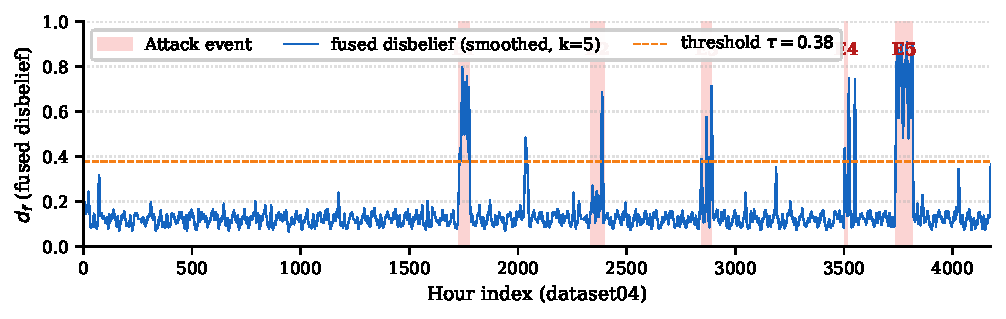
\includegraphics[width=\columnwidth]{fig_batadal_timeseries}
\caption{Fused disbelief $d_f$ over the BATADAL evaluation dataset. Shaded red regions mark attack events E1 to E5. Dashed line is the operating threshold $\tau=0.38$.}
\label{fig:batadal-ts}
\end{figure}

The unsupervised operating points in Table~\ref{tab:batadal-ops} are within 0.04 F1 of the $F_1$-optimal upper bound. The method does not require test-set label access to achieve practical performance.

\textbf{Statistical tests} (Bonferroni-corrected, $n_{\text{comp}}=3$):
Fusion vs.\ no-fusion: $\Delta_{\text{AUROC}}=+0.066$, Cohen's $d=1.01$, $p<10^{-4}$ ($n=152$, large effect).
Historical vs.\ physics strategy: $\Delta_{\text{AUROC}}=+0.089$, $d=1.97$, $p<10^{-4}$ ($n=50$).
Decay vs.\ no-decay: $n=52$, $p=1.0$ (not significant). The negative decay result is honest and informative. For pointwise anomaly detection on BATADAL, exponential decay on $u_f$ does not provide statistically measurable improvement, though rolling-window smoothing does.

\subsection{The SL-Dimension Specificity Finding}

Per-event best-signal analysis (Table~\ref{tab:per-event}, Fig.~\ref{fig:per-event}) reveals that the three SL dimensions detect structurally different attack classes. No single signal maximizes detection across all events.

\begin{table}[t]
\centering
\caption{BATADAL per-event AUROC by SL signal. Best-in-row bolded.}
\label{tab:per-event}
\footnotesize
\begin{tabular}{@{}lcccccc@{}}
\toprule
\textbf{Event} & $u_f$ & $d_f$ & $\max u$ & $\max d$ & $\bar{u}$ & $\alpha u{+}\beta d$ \\
\midrule
1 (42h) & 0.95 & 0.95 & 0.53 & 0.94 & 0.76 & \textbf{0.96} \\
2 (60h) & 0.77 & \textbf{0.81} & 0.57 & 0.73 & 0.68 & 0.80 \\
3 (37h) & 0.42 & 0.48 & 0.50 & \textbf{0.59} & 0.48 & 0.47 \\
4 (7h)  & \textbf{0.84} & 0.68 & 0.45 & 0.49 & 0.71 & 0.70 \\
5 (73h) & \textbf{0.99} & 0.97 & 0.73 & 0.97 & 0.82 & 0.98 \\
\bottomrule
\end{tabular}
\end{table}

\begin{figure}[t]
\centering
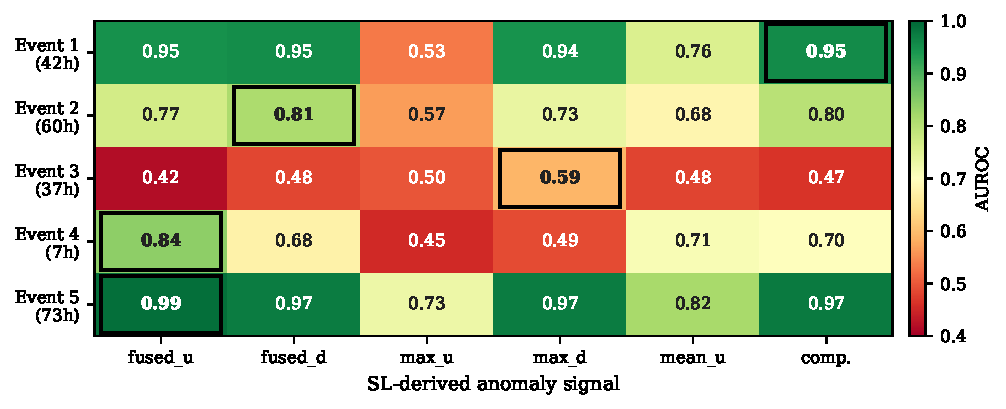
\includegraphics[width=\columnwidth]{fig_per_event_signal}
\caption{Per-event AUROC heatmap across six SL-derived signals. Each row is an attack event; each column is a signal. Best-in-row cells are outlined. No single signal wins on every event.}
\label{fig:per-event}
\end{figure}

Events 4 and 5 (short- and long-duration physical-parameter manipulation) are best detected by fused uncertainty $u_f$. These are anomalies where sensor readings drift outside historical envelopes, elevating $u$.
Events 1 and 2 (value-injection attacks) are best detected by fused disbelief $d_f$ or the composite, which captures attacks where the injected values violate what the pipeline believes possible.
Event 3, a stealth PLC manipulation undetected by most BATADAL baselines, is only weakly detectable via peak disbelief $\max d$: brief contradiction spikes in individual sensors are averaged away by fused metrics. Signal-level inter-comparison reaches statistical significance ($u_f$ vs.\ $d_f$: $p=0.0002$, $d=3.67$).

This is a structural finding. Subjective logic is not a monolithic anomaly detector but a decomposable triple whose components are complementary. A practical deployment should compute all three dimensions and combine them via attack-class-informed rules or learned ensembles.

\subsection{Ablation Across Conditions}

\begin{figure}[t]
\centering
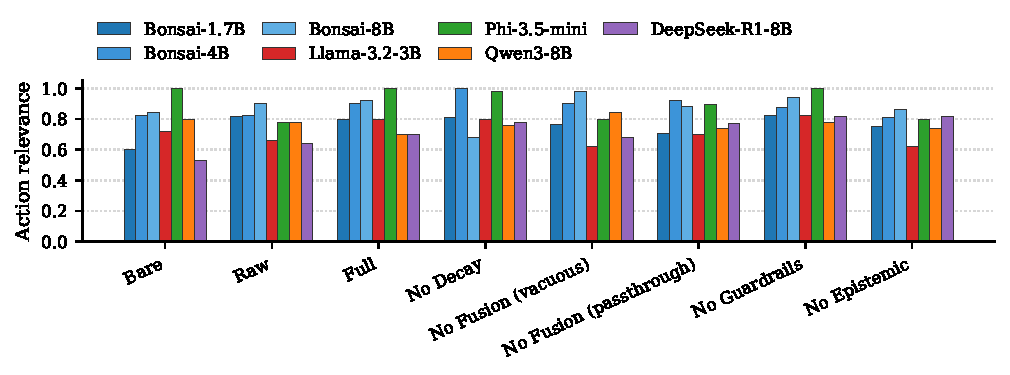
\includegraphics[width=\columnwidth]{fig_ablation}
\caption{Synthetic ablation summary. Action relevance across 8 conditions and 7 models. Condition C (full pipeline) consistently achieves high relevance; removing the epistemic layer (G) uniformly collapses threshold accuracy (not shown here; see Fig.~\ref{fig:safety}).}
\label{fig:ablation}
\end{figure}

Three observations from Fig.~\ref{fig:ablation}:
SL context improves action relevance (A vs.\ C), most dramatically for weaker models.
Temporal decay matters for stale data (C vs.\ D). Aggregate action relevance is similar, but D fails on the \textit{stale alarm} scenario where decay should neutralize an outdated alarm.
Guardrails do not change action relevance (C vs.\ F), as expected. Guardrails filter post-hoc. Their value is in the safety dimension.

\subsection{Limitations}

The synthetic scenarios, while covering five distinct safety patterns, are a controlled evaluation suite and not a deployment on real industrial hardware.
BATADAL Event~3 (stealth attack) remains marginally detectable (AUROC~0.59). No unsupervised method in the published BATADAL literature detects it reliably.
Whitelist accuracy varies across models (0.36 to 0.80 under C), partly reflecting prompt sensitivity rather than a fundamental capability gap.
BATADAL validation here excludes the LLM. Full Tier~1 to 4 validation on BATADAL is the focus of ongoing work.

%% ======================================================================
\section{Conclusion}
%% ======================================================================

Epistemic Edge is a reusable neuro-symbolic pipeline that integrates subjective-logic uncertainty quantification with LLM-driven IoT actuation. A synthetic ablation across seven models and 2{,}800 trials shows that epistemic guardrails, grounded in calibrated SL fusion, are a necessary complement to behavioral guardrails. Without them, threshold accuracy collapses to 0.40. Real-data validation on BATADAL achieves AUROC~0.9004 without supervised training, matching competitive trained methods. A structural finding is that the three SL dimensions detect qualitatively different attack classes, suggesting future work combining them via attack-class-aware decision rules.

We also provide the first IoT-actuation evaluation of PrismML Bonsai 1-bit models. Bonsai-8B at 1-bit outperforms Qwen3-8B at 4-bit on action relevance while requiring half the storage.

Future work will complete the Tier~1 to 4 BATADAL validation with LLM in the loop, extend to SWaT~\cite{goh2017swat}, deploy on edge hardware, and investigate learned ensembles over the three SL dimensions.

All code, experiment scripts, and results are publicly available.\footnote{Repository URL withheld for double-blind review.}

\balance
\bibliographystyle{IEEEtran}
\bibliography{references}

\end{document}
